%% Template para dissertacao/tese na classe UFBAthesis
%% versao 1.0
%% (c) 2005 Paulo G. S. Fonseca
%% (c) 2012 Antonio Terceiro
%% (c) 2014 Christina von Flach
%% www.dcc.ufba.br/~flach/ufbathesis

%% Carrega a classe ufbathesis
%% Opcoes: * Idiomas
%%           pt   - portugues (padrao)
%%           en   - ingles
%%         * Tipo do Texto
%%           bsc  - para monografias de graduacao
%%           msc  - para dissertacoes de mestrado (padrao)
%%           qual - exame de qualificacao de mestrado
%%           prop - exame de qualificacao de doutorado
%%           phd  - para teses de doutorado
%%         * Media
%%           scr  - para versao eletronica (PDF) / consulte o guia do usuario
%%         * Estilo
%%           classic - estilo original a la TAOCP (deprecated) - apesar de deprecated, manter esse.
%%           std     - novo estilo a la CUP (padrao)
%%         * Paginacao
%%           oneside - para impressao em face unica
%%           twoside - para impressao em frente e verso (padrao)

% Atenção: Manter 'classic' na declaracao abaixo:
\documentclass[pt, bsc, classic, a4paper]{ufbathesis}

%% Preambulo:
%% Preambulo:

\usepackage[utf8]{inputenc}
\usepackage{graphicx}
\usepackage{lipsum}
\usepackage{hyphenat}
\usepackage[dvipsnames, table]{xcolor}
\usepackage{booktabs}
\usepackage{pifont}
\usepackage{multirow}
\usepackage{listings} 
\usepackage{colortbl}
\usepackage{xfrac}
% \usepackage[FIGTOPCAP]{subfigure}
\usepackage[printonlyused, withpage]{acronym}

%% BEGIN - modificacoes de Andre Madureira

% pseudocode / algorithms / source code
\usepackage{algorithm}
\usepackage{algpseudocode}

% source code
\usepackage{listings}           
\usepackage{caption}

% make all the sections uppercase
\usepackage{sectsty}

% define arial font as the default font
% \usepackage[scaled=0.92]{helvet} 
% \renewcommand{\familydefault}{\sfdefault}
% \sectionfont{\sfdefault}
% \subsectionfont{\sfdefault}
% \subsubsectionfont{\sfdefault}
% \paragraphfont{\sfdefault}

% \usepackage{datatool} % allow sorting algorithms

\usepackage{caption, subcaption, float, url} % text and images
\usepackage{tabularx} % tables
\usepackage{amsmath, amsfonts, amssymb, bbm} % allow math expressions
\usepackage[brazil]{babel} % define charset to support brazilian portuguese (dictionary as well)
\usepackage[T1]{fontenc}
\usepackage{enumitem, csquotes, microtype}
\renewcommand{\mkcitation}[1]{ #1} %format csquotes citation

% allow custom indentation
\setlist[description]{leftmargin=0cm,labelindent=0.7cm}

% indentation of the paragraph
\usepackage{indentfirst}    % first line indent
\setlength{\parindent}{1.25cm} % set indentation space
% \setlength{\parskip}{1em} % space between paragraphs

% set source code formatting
\definecolor{codegreen}{rgb}{0,0.6,0}
\definecolor{backcolour}{rgb}{0.95,0.95,0.92}
\definecolor{codegray}{rgb}{0.5,0.5,0.5}
\lstset{
  backgroundcolor=\color{backcolour},  % background of the code
  commentstyle=\color{codegreen},      % comments style
  numberstyle=\small\color{codegray}\textbf,  % line number style / color
%   basicstyle=\defaultfontsize,
  %numberstyle=\small,       defaultfontsize      % adjust the size of numbers
  numbers=left,                     % show numbers to the left
  captionpos=b,                     % sets the caption-position to bottom
  numbersep=7pt,                 % how far the line-numbers are from the code  
  showtabs=false,                  % show tabs within strings adding particular underscores
  stepnumber=1,                   % the step between two line-numbers. If it's 1, each line will be numbered
  tabsize=4,	                        % sets default tabsize to 2 spaces
  xleftmargin=0.6cm,            % adjust left margin
  breaklines=true,
  postbreak=\mbox{\textcolor{red}{$\hookrightarrow$}\space},  
  extendedchars=true,
  literate={á}{{\'a}}1 {â}{{\^a}}1 {ã}{{\~a}}1 {Á}{{\'A}}1 {Â}{{\^A}}1 {Ã}{{\~A}}1 {é}{{\'e}}1 {ê}{{\^e}}1 {ẽ}{{\~e}}1 {É}{{\'E}}1 {Ê}{{\^E}}1 {Ẽ}{{\~E}}1 {ô}{{\^o}}1 {õ}{{\~o}}1 {ó}{{\'o}}1 {Ô}{{\^O}}1 {Õ}{{\~O}}1 {Ó}{{\'O}}1 {í}{{\'i}}1 {Í}{{\'I}}1 {ú}{{\'u}}1 {Ú}{{\'U}}1 {ç}{{\c{c}}}1,
}
% create diff language
\definecolor{diffstart}{rgb}{ 0.00,  0.55, 0.83}
\definecolor{diffincl}{rgb}{  0.00,  0.55, 0.00}
\definecolor{diffrem}{rgb}{   1.00,  0.30, 0.00}
\lstdefinelanguage{diff}{
%     basicstyle=\ttfamily,
    morecomment=[f][\color{diffstart}\textbf]{@@},
    morecomment=[f][\color{diffincl}]{+},
    morecomment=[f][\color{diffrem}]{-},
    morecomment=[f][\color{diffincl}\textbf]{+++},
    morecomment=[f][\color{diffrem}\textbf]{---}    
  }
%   create conf language
\lstdefinelanguage{conf}{
	sensitive = true,
    keywords={config, option},	
    stringstyle=\color{red},
    morecomment=[f]{\#},    
    morestring=[b]{\'},
    morestring=[b]{\"}
}
% caption to code
\renewcommand{\lstlistingname}{Script}% set caption name
\renewcommand{\lstlistlistingname}{Lista de \lstlistingname s}
% set caption format
\DeclareCaptionFont{white}{ \color{white} }
\DeclareCaptionFormat{listing}{
  \colorbox[cmyk]{0.43, 0.35, 0.35,0.01 }{
    \parbox{\textwidth}{\hspace{15pt}#1#2#3}
  }
}
\captionsetup[lstlisting]{ format=listing, labelfont=white, textfont=white, singlelinecheck=false, margin=0pt, font={bf,footnotesize} }  

% load codes from code/ path
\lstset{inputpath=code}

%load images from images/ path
\graphicspath{ {images/} }

%% END - modificacoes de Andre Madureira

% Entidade/Orgão
\entity{Ministério da Educação}

% Universidade
\university{Instituto Federal de Educação, Ciência e Tecnologia da Bahia}

% Endereco (cidade)
\address{Valença}

% Instituto ou Centro Academico
% \institute{}

% Campus
\campus{\textit{Campus} Valença}

% Nome da biblioteca - usado na ficha catalografica
\library{NOME DA BIBLIOTECA AQUI}

% Programa de pos-graduacao
\program{Curso de Tecnologia em Análise e Desenvolvimento de Sistemas}

% Grau
\degree{Tecnólogo}

% Area de titulacao
\majorfield{Análise e Desenvolvimento de Sistemas}

% Titulo da dissertacao
\title{TITULO DA MONOGRAFIA AQUI}

% Data da defesa
\date{2024}
\defenseyear{2024}

% Autor
% e.g. \author{Jose da Silva}
\author{NOME DO ALUNO AQUI}

% Orientador(a)
% Opcao: [f] - para orientador do sexo feminino
% e.g. \adviser[f]{Profa. Dra. Maria Santos}
\adviser{Prof. Dr. xxx (NOME DO ORIENTADOR AQUI)}

% Orientador(a)
% Opcao: [f] - para orientador do sexo feminino
% e.g. \coadviser{Prof. Dr. Pedro Pedreira}
% Comente se nao ha co-orientador
\coadviser{Prof. Dr. xxx (NOME DO COORIENTADOR AQUI)}

%% Inicio do documento
\begin{document}

%% CAPA
\pgcompfrontpage

%% Parte pre-textual
\frontmatter

%% CONTRA-CAPA
\pgcomppresentationpage

%%%%%%%%%%%%%%%%%%%%%%%%%
% Ficha catalografica
%%%%%%%%%%%%%%%%%%%%%%%%%


%%%%%%%%%%%%%%%%%%%%%
% Ficha Catalografica
%%%%%%%%%%%%%%%%%%%%%

\authorcitationname{SOBRENOME, NOME ALUNO} % e.g. Terceiro, Antonio Soares de Azevedo
\advisercitationname{SOBRENOME, NOME ORIENTADOR} % e.g. Chavez, Christina von Flach Garcia
\coadvisercitationname{SOBRENOME, NOME COORIENTADOR} % e.g. Mendonca, Manoel Gomes de
\catalogtype{Disserta\c{c}\~{a}o (Trabalho de Conclusão de Curso)} % e.g. ou ``Tese (Doutorado)''

\catalogtopics{1. PALAVRA CHAVE. 2. PALAVRA CHAVE. 3. PALAVRA CHAVE. 4. PALAVRA CHAVE. 5. PALAVRA CHAVE.} % Listar palavras-chave do trabalho para a FICHA CATALOGRAFICA}, por exemplo, ``1. Complexidade Estrutural. 2. Qualidade de Software 3. Engenharia de Software''
\catalogcdd{XXX.XX} % e.g.  XXX.XX (número nesse formato serah dado pela biblioteca)
\catalogcdu{XXX.XX.XXX} % e.g.  XXX.XX.XXX (idem) 
\catalogingsheet

%%%%%%%%%%%%%%%%%%%%%
% Termo de aprovacaoo
%%%%%%%%%%%%%%%%%%%%%


%%%%%%%%%%%%%%%%%%%%%
% Termo de aprovacaoo
%%%%%%%%%%%%%%%%%%%%%

\approvalsheet{DIA de MES de 2024}{
   \comittemember{Profa. Dra. Professora 1}{Universidade XYZ}
   \comittemember{Prof. Dr. Professor 2}{Universidade 123}
   \comittemember{Profa. Dra. Professora 3}{Universidade ABC}
   % Para mestrado, apenas 3.
   \comittemember{Prof. Dr. Professor 4}{Universidade HJKL}
   \comittemember{Profa. Dra. Professora 5}{Universidade QWERTY}
}

%%%%%%%%%%%%%%%%%%%%%%%%%%%%%%%%%%%%%%%%
% Dedicatoria, Agradecimentos, Epigrafe
%%%%%%%%%%%%%%%%%%%%%%%%%%%%%%%%%%%%%%%%

% Dedicatoria
%% DEDICATORIA

\begin{dedicatory}
Folha opcional em que o(a) autor(a) homenageia pessoas e/ou instituições, dedicando-lhes seu trabalho.
\end{dedicatory}

% Agradecimentos
%% Agradecimentos

\acknowledgements
Folha opcional, contendo em forma de texto ou de lista os nomes de pessoas ou instituições que contribuíram de forma relevante para o trabalho.

% Epigrafe

%% Epigrafe

\begin{epigraph}[TITULO AQUI]{AUTOR AQUI}
\setstretch{1.0}
Inscrição ou frase alusiva ao tema do trabalho, de caráter opcional, com a citação da fonte de onde foi extraída, a qual deve constar na lista de referências.\\
\end{epigraph}

%%%%%%%%%%%%%%%%%%%%%
% Resumos em Portugues e Ingles
%%%%%%%%%%%%%%%%%%%%%

%%%%%%%%%%%%%%%%%%%%%
% Resumo em Portugues
%%%%%%%%%%%%%%%%%%%%%

\resumo

Resumo é a “Apresentação concisa dos pontos relevantes de um texto”, isto é, natureza do trabalho, contexto, objetivos, metodologia, resultados e conclusões.

Deve ser redigido na terceira pessoa do singular, com o verbo na voz ativa, em frases correntes, sem enumeração de tópicos. A frase de abertura deve explicitar o tema do trabalho. Deve ser evitado o uso de frases negativas, parágrafos, fórmulas, siglas, símbolos, citações bibliográficas. É encabeçado pela palavra RESUMO em negrito e letras maiúsculas, centralizada ao alto, com o texto em espaço simples e justificado. Ao final, deve incluir as palavras-chave representativas do conteúdo.

% Palavras-chave do resumo em Portugues
\begin{keywords}
 PALAVRA CHAVE. PALAVRA CHAVE. PALAVRA CHAVE. PALAVRA CHAVE. PALAVRA CHAVE.
\end{keywords}
%%%%%%%%%%%%%%%%%%%
% Resumo em Ingles
%%%%%%%%%%%%%%%%%%%

\abstract

Versão do Resumo para o inglês

% Palavras-chave do resumo em Ingles
\begin{keywords}
 PALAVRA CHAVE.  PALAVRA CHAVE.  PALAVRA CHAVE. PALAVRA CHAVE . PALAVRA CHAVE.
\end{keywords} 

%% LISTA DE SIGLAS (ACRONIMOS)

%% LISTA DE SIGLAS (ACRONIMOS)

\chapter*{Lista de Siglas}

% Sintaxe da lista de acordo com a documentação do pacote `acronym'
% documentação: http://mirror.unl.edu/ctan/macros/latex/contrib/acronym/acronym.pdf
\begin{acronym}[PGCOMP]
    \acro{API}{\textit{Application Programming Interface}}           
    \acro{CNPq}{Conselho Nacional de Desenvolvimento Científico e Tecnológico}
    \acro{CPqD}{\textit{Software Switch} CPqD}     
    \acro{CPU}{\textit{Central Processor Unit}}   	 
    \acro{IFBA}{Instituto Federal de Educação, Ciência E Tecnologia da Bahia}   	 
    \acro{WMN}{\textit{Wireless Mesh Network}}        
\end{acronym} 

%% LISTA DE FIGURAS
% Comente para ocultar
\listoffigures

%% LISTA DE TABELAS
% Comente para ocultar
\listoftables

%% LISTA DE SCRIPTS
% Comente para ocultar
\lstlistoflistings

%%%%%%%%%%%%%%%%%%%
% Sumario / Indice
%%%%%%%%%%%%%%%%%%%

%% SUMARIO
% Comente para ocultar
\tableofcontents

%% Parte textual
\mainmatter

% Eh aconselhavel criar cada capitulo em um arquivo separado, digamos
% "capitulo1.tex", "capitulo2.tex", ... "capituloN.tex" e depois
% inclui-los com:
% \include{capitulo1}
% \include{capitulo2}
% ...
% \include{capituloN}
%
% Importante: 
% Use \xchapter{}{} ao inves de \chapter{}; se não quiser colocar texto antes do inicio do capitulo, use \xchapter{texto}{}.

% DICAS DO USO DO LATEX (comentar quando for usar o modelo)

\xchapter{\MakeTextUppercase{Dicas do LaTeX}}{}

\section{Citações}
 
Para realizar a citação de um trabalho, basta usar o comando \verb|\cite{referencia}|. Caso a citação faça parte do texto, ela deve ser feita usando o comando \verb|\citeonline{referencia}|. Exemplos:

Uma interface deve estar bem projetada \cite{autor2023}.

Segundo \citeonline{fulano2024}, os sistemas computacionais [...]

\textbf{IMPORTANTE}: Para as citações funcionarem, você precisa inserir as referencias no arquivo \textbf{capitulos/biblio.bib}, seguindo o formato BibTeX. 

\subsection{Citações Diretas}

Para fazer uma citação direta, basta usar o comando \verb|\blockquote[{citacao}]{texto}|. 

\textbf{Exemplo}: \blockquote[{\cite{fulano2024}}]{Este é um exemplo de citação direta de um texto curto.} 

Caso o texto ocupe muitas linhas, o mesmo comando \verb|\blockquote| ira fazer a formatação automaticamente para você. \textbf{Exemplo}:

\blockquote[{\cite{fulano2024}}]{Este é um exemplo de citação longa, onde o texto é destacado do restante do conteúdo. \lipsum[1]}

\section{Acronimos}

Para usar uma sigla/acronimo no texto, você precisa inserir ele no arquivo \textbf{pretextuais/siglas.tex} e depois usar o comando \verb|\ac{sigla}|. No primeiro uso da sigla, o LaTeX vai expandir ela para a sua forma por extenso, seguida de parentese. Nos usos subsequentes, o LaTeX irá usar apenas a sigla. Se você quiser usar a sigla no plural, você deve utilizar o comando \verb|\acp{sigla}|. Veja os exemplos abaixo:

Sistemas computacionais possuem uma \ac{CPU} e interagem uns com os outros usando uma \ac{API}. Uma \ac{API} é uma interface de programação padronizada. Multiplas \acp{API} podem ser utilizadas para compor sistemas complexos.

\textbf{LEMBRE-SE}: Toda palavra em inglês deve estar em itálico pelas normas da ABNT. Para isso use o comando \verb|\textit{texto aqui}|.

\section{Itemização}

Você pode criar itemizações com \textit{bullets}:

\begin{itemize}
    \item Um topico
    \item outro topico
    \item ultimo topico
\end{itemize}

\subsection{Enumeração}

Tambem podemos criar itemizações com numeração:

\begin{enumerate}    
    \item item X
    \item item A
    \item item Z       
\end{enumerate}

\section{Seções}

Para organizar melhor seu texto, utilize os comandos abaixo para criar seções e subseções:

\begin{verbatim}
    \section{NOME_SECAO}
    \subsection{NOME_SUBSECAO}
    \subsubsection{NOME_SUBSUBSECAO}
    \paragraph{NOME_PARAGRAFO}
\end{verbatim}

\section{Figuras}

Para citar uma figura no texto, você deve usar o texto ``Figura'' seguido do comando \verb|~\ref{id_figura}|. Veja exemplo abaixo.

Na Figura~\ref{fig:id_figura}, vemos como é feita a configuração de um firewall dentro de um \textit{switch} OpenWRT.

\textbf{IMPORTANTE}: Não devemos usar termos como ``abaixo'' ou ``acima'' no texto que se refere a figura, pois quem ira posicionar a figura no PDF é o LaTeX! Logo não temos como ter certeza de onde a figura sera posicionada.

\begin{figure}[!htb]
    \centering
    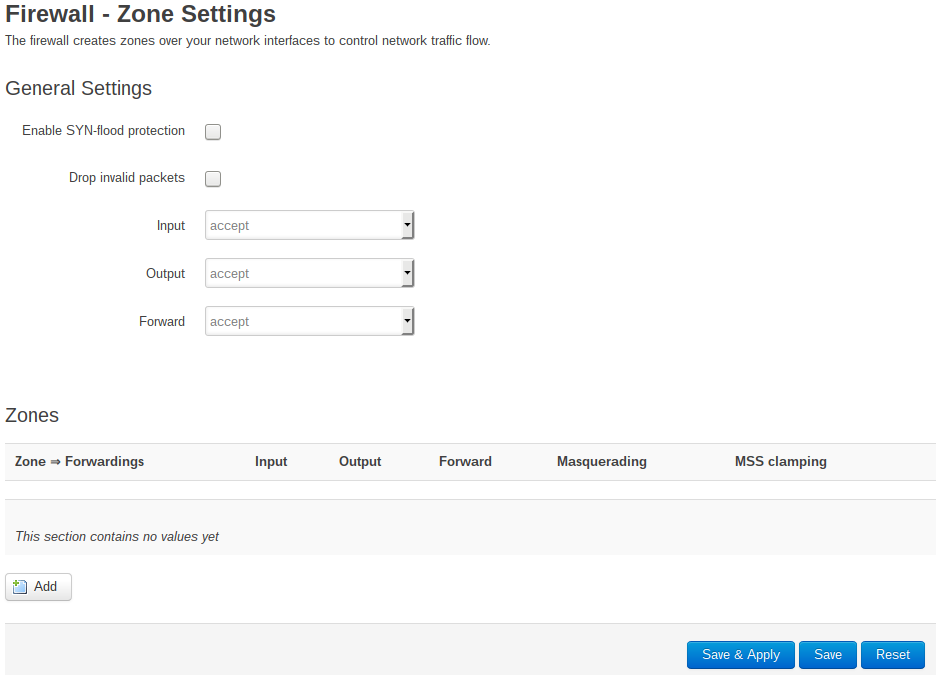
\includegraphics[width=\textwidth]{images/firewall_zone}
    \caption{Legenda da figura}
    \label{fig:id_figura}    
\end{figure}

\subsection{Subfiguras}

É uma técnica para posicionar várias figuras juntas, como subitens de uma figura maior. Elas podem ser posicionadas lado-a-lado ou uma abaixo da outra. Veja exemplo abaixo.

\begin{figure}[!htb]
    \centering
    % Primeira subfigura
    \begin{subfigure}[b]{0.45\textwidth}
        \centering
        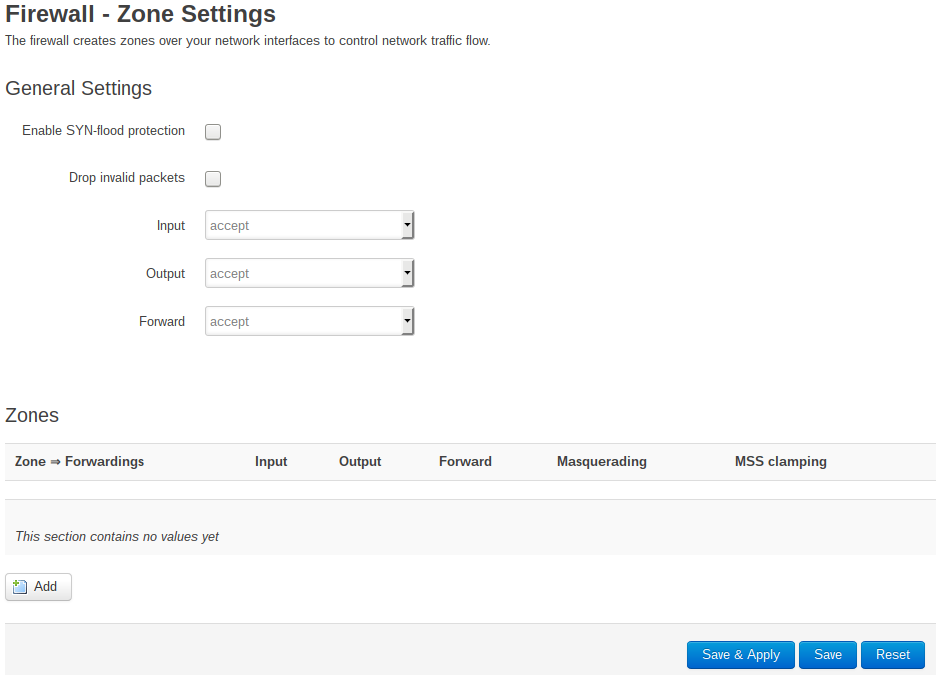
\includegraphics[width=\textwidth]{images/firewall_zone}
        \caption{Legenda da Subfigura 1}
        \label{fig:id_subfig1}
    \end{subfigure}
    \hfill
    % Segunda subfigura
    \begin{subfigure}[b]{0.45\textwidth}
        \centering
        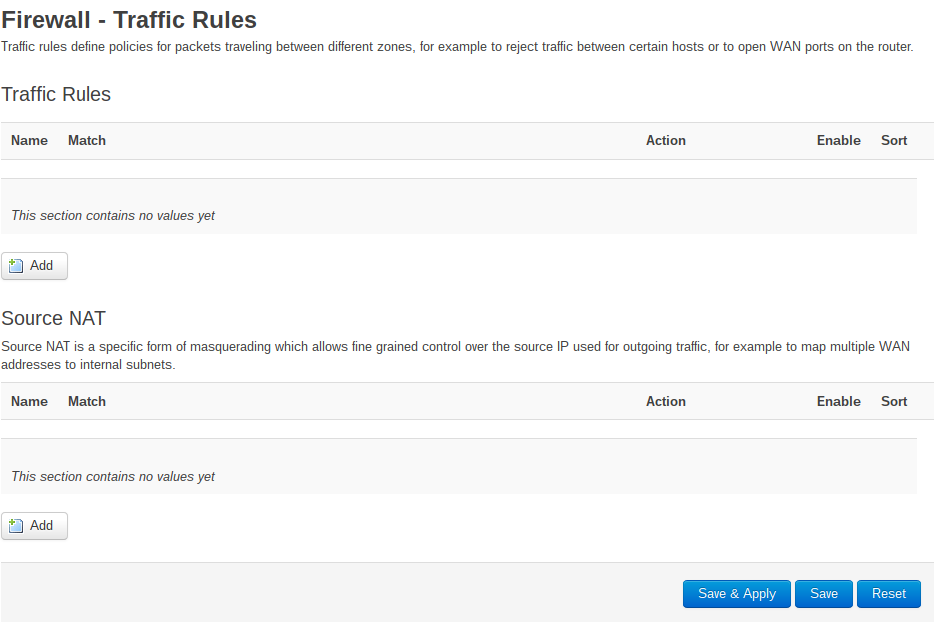
\includegraphics[width=\textwidth]{images/firewall_traffic.png}
        \caption{Legenda da Subfigura 2}
        \label{fig:id_subfig2}
    \end{subfigure}
    \caption{Legenda da Figura Principal (exemplo lado-a-lado)}
    \label{fig:id_figura_principal}
\end{figure}

\section{Tabelas}

\verb@\begin{tabular}{|c|c|c|}@: Cria uma tabela com três colunas centralizadas (c), com bordas verticais entre elas.

\verb@\multicolumn{2}{|c|}{Texto}@: Mescla duas colunas (2) e as alinha centralizadas (c), com bordas verticais ao redor.

\verb|\multirow{2}{*}{Texto}|: Mescla duas linhas (2), ocupando uma única célula na coluna, e alinha o texto ao centro verticalmente (padrão). O * permite que a largura da célula seja ajustada automaticamente.

\verb|\hline|: Insere uma linha horizontal.

\verb|\cline{2-3}|: Desenha uma linha horizontal que cobre apenas as colunas 2 e 3, usada para delinear células não mescladas.

\begin{table}[!htb]
\centering
\begin{tabular}{|c|c|c|}
\hline
Coluna 1 & Coluna 2 & Coluna 3 \\
\hline
Dado 1   & Dado 2   & Dado 3   \\
\hline
Dado 4   & Dado 5   & Dado 6   \\
\hline
Dado 7   & Dado 8   & Dado 9   \\
\hline
\end{tabular}
\caption{Exemplo de Tabela Simples}
\label{tab:tabela_simples}
\end{table}

\subsection{Tabelas com celulas mescladas (horizontal)}

Exemplo de tabela com celulas mescladas na horizontal:

\begin{table}[!htb]
\centering
\begin{tabular}{|c|c|c|}
\hline
Coluna 1 & \multicolumn{2}{|c|}{Colunas 2 e 3 Mescladas} \\
\hline
Dado 1 & Dado 2 & Dado 3 \\
\hline
\multicolumn{2}{|c|}{Células 1 e 2 Mescladas} & Dado 6 \\
\hline
Dado 7  & \multicolumn{2}{|c|}{Células 2 e 3 Mescladas} \\
\hline
\end{tabular}
\caption{Exemplo de Tabela com Células Mescladas Horizontalmente}
\label{tab:tabela_horizontal}
\end{table}

\subsection{Tabelas com celulas mescladas (vertical)}

Exemplo de tabela com celulas mescladas na vertical:

\begin{table}[!htb]
\centering
\begin{tabular}{|c|c|c|}
\hline
\multirow{2}{*}{Célula Mesclada na Vertical} & Coluna 2 & Coluna 3 \\ 
\cline{2-3}
         & Dado 2   & Dado 3   \\
\hline
Dado 4   & Dado 5   & Dado 6   \\
\hline
Dado 7   & Dado 8   & Dado 9   \\
\hline
\end{tabular}
\caption{Exemplo de Tabela com Células Mescladas Verticalmente}
\label{tab:tabela_vertical}
\end{table}

\section{Notas de Rodapé}

Texto com nota de rodapé.\footnote{Este é um exemplo de nota de rodapé.}

\section{Pseudocódigo}

O Algoritmo~\ref{alg:id_algoritmo} do pseudocodigo segue abaixo:

\begin{algorithm}
\caption{Algoritmo de Exemplo com IF e FOR}
\label{alg:id_algoritmo}
\begin{algorithmic}[1] % O [1] indica que as linhas serão numeradas
    \State $a \gets 0$ \Comment{Inicializa a variável $a$ com 0}
    \State $b \gets 1$ \Comment{Inicializa a variável $b$ com 1}
    \State $n \gets 10$ \Comment{Define o número de iterações do loop}
    
    \For{$i \gets 1$ \textbf{to} $n$} \Comment{Inicia um loop de 1 até $n$}
        \If{$a < b$} \Comment{Condição IF: verifica se $a$ é menor que $b$}
            \State $c \gets a + b$ \Comment{Se a condição for verdadeira, calcula $c = a + b$}
        \Else
            \State $c \gets a - b$ \Comment{Se a condição for falsa, calcula $c = a - b$}
        \EndIf
        \State $a \gets b$ \Comment{Atualiza $a$ para o valor de $b$}
        \State $b \gets c$ \Comment{Atualiza $b$ para o valor de $c$}
    \EndFor

    \State \textbf{return} $b$ \Comment{Retorna o valor final de $b$}
\end{algorithmic}
\end{algorithm}

\section{Código Python}

O Script~\ref{lst:id_codigo_python} segue abaixo:

\begin{lstlisting}[language=Python, caption={Exemplo de Código Python}, frame=single, label={lst:id_codigo_python}]
# Este é um exemplo de código Python
def fibonacci(n):
    """Retorna a sequência de Fibonacci até n."""
    a, b = 0, 1
    while a < n:
        print(a, end=' ')
        a, b = b, a + b
    print()

# Chama a função com n = 1000
fibonacci(1000)
\end{lstlisting}



% % INTRODUCAO

%% INTRODUCAO

\xchapter{\MakeTextUppercase{Introdu\c{c}\~{a}o}}{}

Uma introdução de TCC deve incluir os seguintes elementos, geralmente escritos na forma de texto corrido (orações e paragrafos), evitando itemizações ou enumerações:

\begin{itemize}
    \item \textbf{Contextualização}: Apresentação do tema e sua relevância no contexto acadêmico ou social.        
    \item \textbf{Problema de Pesquisa}: Definição clara da questão ou problema que o trabalho pretende investigar.
    \item \textbf{Justificativa}: Explicação da importância do estudo e das contribuições esperadas.
    \item \textbf{Metodologia}: Breve descrição dos métodos e abordagens utilizados na pesquisa.    
\end{itemize}

\textbf{SUGESTÃO}: É preferivel elaborar a introdução no final do trabalho, após ter redigido todas os outros capítulos. Dessa forma, você terá uma visão panorâmica do trabalho, o que permite que você construa a sua introdução como um resumo do conteúdo das demais seções.

\section{OBJETIVOS}

\subsection{\MakeTextUppercase{GERAL}}
Descrever, de maneira geral, o que se deseja alcançar com a proposta descrita na monografia. O objetivo geral é geralmente descrito como um paragrafo simples, que começa com um verbo no imperativo. O verbo deve ser passivel de avaliação nos resultados.

\subsection{\MakeTextUppercase{ESPECÍFICOS}}
Descrever, de maneira detalhada, como o objetivo geral será alcançado, na forma de topicos. Cada objetivo deve começar com um verbo no imperativo, que possa ser avaliado nos resultados.

\begin{itemize}
\item objetivo 1
\item objetivo 2
\item objetivo 3
\end{itemize}

\section{ORGANIZAÇÃO DO TRABALHO}

Esta subseção contem uma breve descrição dos capítulos ou seções que compõem o TCC, indicando a organização do conteúdo da monografia.



% REFERENCIAL TEORICO

%% REFERENCIAL TEORICO

\xchapter{\MakeTextUppercase{Revis\~{a}o Bibliogr\'{a}fica}}{}

Uma revisão bibliográfica de TCC deve incluir os seguintes elementos, geralmente escritos como texto corrido (orações e paragrafos), evitando itemizações ou enumerações:

\begin{itemize}
    \item \textbf{Fundamentação Teórica}: Apresentação das principais teorias, conceitos e autores relevantes para o tema.
    \item \textbf{Análise Crítica}: Discussão das contribuições e limitações das obras consultadas, evidenciando lacunas e pontos de divergência na literatura.
    \item \textbf{Evolução do Tema}: Descrição do desenvolvimento histórico e das tendências recentes na área de estudo.
    \item \textbf{Relacionamento com a Pesquisa}: Explicação de como os estudos revisados se conectam com a pesquisa realizada, justificando a escolha do referencial teórico.
    \item \textbf{Síntese}: Resumo dos principais insights e direcionamentos que a revisão proporciona ao trabalho.
\end{itemize}

\textbf{IMPORTANTE}: Tudo que for mencionado na revisão bibliografica, que não tenha sido fruto deste trabalho de TCC, \textbf{deve estar devidamente citado}, a fim de evitar plágio e autoplágio (\url{https://www2.ufjf.br/ppgedumat/discentes/plagio-e-autoplagio/}).

% % METODOLOGIA

\xchapter{\MakeTextUppercase{Metodologia}}{} %sem preambulo

A metodologia descreve o caminho que culminou nos resultados encontrados no TCC, permitindo assim a replicação do estudo por outro pesquisador. Desta forma, a metodologia de um TCC deve incluir os seguintes elementos, geralmente escritos na forma de texto corrido (orações e paragrafos), evitando itemizações ou enumerações:

\begin{itemize}
    \item \textbf{Tipo de Pesquisa}: Definição do tipo de estudo (quantitativo, qualitativo, exploratório, descritivo, etc.).
    \item \textbf{Objeto de estudo}: Descrição do fenômeno, evento, processo, grupo, software ou sistema que está sendo investigado.
    \item \textbf{Procedimentos de Coleta de Dados}: Descrição das técnicas e instrumentos utilizados para coleta de dados (questionários, entrevistas, experimentos, etc.).
    \item \textbf{População e Amostra}: Explicação do universo de estudo e dos critérios de seleção da amostra.
    \item \textbf{Análise de Dados}: Métodos e técnicas utilizados para analisar os dados coletados (estatística, análise de conteúdo, etc.).
    \item \textbf{Aspectos Éticos}: Considerações sobre a ética na pesquisa, como consentimento informado e confidencialidade.
\end{itemize}

% % RESULTADOS / DISCUSSAO

%% DISCUSSAO

\xchapter{\MakeTextUppercase{Discussão de Resultados}}{} %sem preambulo

Este capítulo deve incluir os seguintes elementos, geralmente escritos na forma de texto corrido (orações e paragrafos), evitando itemizações ou enumerações:

\begin{itemize}
    \item \textbf{Apresentação dos Resultados}: Exposição clara dos dados coletados utilizando tabelas, gráficos, e figuras para facilitar a compreensão.
    \item \textbf{Interpretação dos Resultados}: Análise dos dados à luz do referencial teórico e dos objetivos do estudo, destacando os principais achados e quais objetivos foram alcançados.
    \item \textbf{Discussão Comparativa}: Comparação dos resultados obtidos com outros estudos relevantes na literatura, apontando semelhanças, diferenças e possíveis explicações.
    \item \textbf{Implicações dos Resultados}: Reflexão sobre as contribuições teóricas, práticas e/ou sociais dos resultados, indicando sua relevância e aplicação.
\end{itemize}



% % CONCLUSAO

% CONCLUSAO

\xchapter{\MakeTextUppercase{Conclus\~{a}o}}{} %sem preambulo

Este capítulo deve incluir os seguintes elementos, na forma de texto corrido (orações e paragrafos), sem itemizações ou enumerações:

\begin{itemize}
    \item \textbf{Síntese dos Resultados}: Resumo dos principais achados da pesquisa, respondendo diretamente ao problema de pesquisa e aos objetivos propostos.
    \item \textbf{Contribuições}: Indicação das contribuições do estudo para o campo acadêmico, profissional ou social, destacando sua relevância.
    \item \textbf{Limitações do Estudo}: Reconhecimento das limitações enfrentadas durante a pesquisa e como elas podem ter impactado os resultados.
    \item \textbf{Sugestões para Pesquisas Futuras}: Recomendações para estudos futuros que possam aprofundar ou expandir as questões abordadas.
    \item \textbf{Considerações Finais}: Reflexões finais sobre a importância do estudo, ressaltando a originalidade e as principais implicações.
\end{itemize}

\textbf{IMPORTANTE}: A conclusão não deve conter conteúdo novo. Ela deve servir como um compilado geral do trabalho, geralmente escrita na forma de alguns poucos parágrafos.


%% Parte pos-textual (REFERENCIAS BIBLIOGRAFICAS)
\backmatter

% Bibliografia
% É aconselhável utilizar o BibTeX a partir de um arquivo, digamos "biblio.bib".
% Para ajuda na criação do arquivo .bib e utilização do BibTeX, recorra ao
% BibTeXpress em www.cin.ufpe.br/~paguso/bibtexpress
\bibliographystyle{abntex2-alf}
\bibliography{capitulos/biblio}

%%%%%%%%%%%%
%%    Apendices  %%
%%%%%%%%%%%%

% Comente se nao houver apendices
% \appendix

% Eh aconselhavel criar cada apendice em um arquivo separado, digamos
% "apendice1.tex", "apendice.tex", ... "apendiceM.tex" e depois
% inclui--los com:


%% APENDICE A

\xchapter{EXEMPLO DE APÊNDICE}{} %sem preambulo
\lipsum[1-5]


%% Fim do documento
\end{document}
%------------------------------------------------------------------------------------------%
